\section{Induction}
\subsection{Alimentation}
Le circuit d'induction partage la même alimentation que celle du module du code manchester soit (5V/3A).
\subsection{Pont H}
On utilise un pont H afin d'induire un grand courant alternatif dans la bobine du primaire. La fréquence de ce courant est dicté par un PWM généré par le Arduino Uno qui sera aussi situé à la station de base.

\subsection{Tramsformateur}
Le rapport de transformation entre la bobine primaire et celle du secondaire est d'environ 1:1.2. Ce rapport à été choisi de façon à ce que la bobine du secondaire ait elle aussi un tension d'environ 5V.
En effet, le pont H alimenté par du (0-5V) subit une chute de tension de 0.7V causé par les transistors c'est pourquoi il nous faut compenser cet effet par un nombre de tour plus élevé au secondaire
qu'au primaire. Pour l'instant, le calibre de fils choisi pour nos deux bobines est le AWG 25, cependant il risque d'être changé lors de lors de l'optimisation.
\subsection{Choix des coeurs de férite}
Afin de faciliter l'enlignement des deux bobines, nous avons choisi de prendre des coeurs de férrite de 3,5cm de diamètre.
En effet, bien que des coeurs ferrite ayant un diamètre plus petit aurait permis de concentrer d'avantage les lignes de champs magnétique, l'enlignement de ces derniers auraient été un énorme fardeau pour
la vision.


\subsection{Circuit d'induction}


  \begin{figure}[H]
    \label{drive}
    \centering
    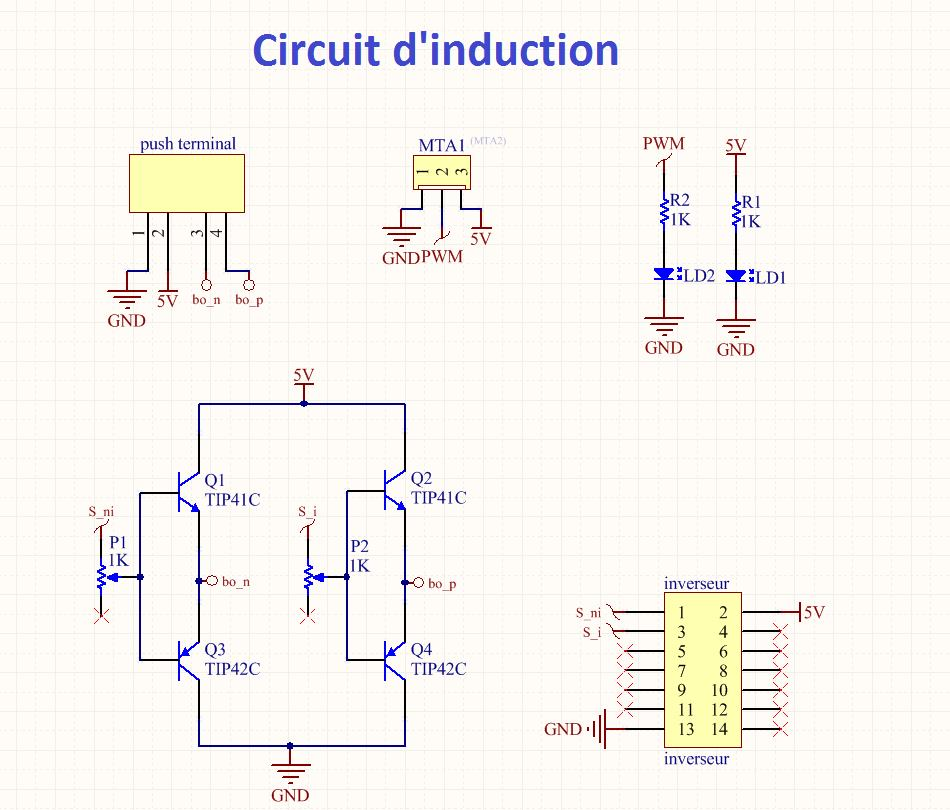
\includegraphics[scale=0.4]{resources/induction.jpg}
    \caption{Circuit d'induction de la bobine}
  \end{figure}
